% REMOVED COMMENTS HERE
\input{removedComments/1.tex}
% REMOVED COMMENTS HERE

\documentclass[journal]{IEEEtran}

% REMOVED COMMENTS HERE
\input{removedComments/2.tex}
% REMOVED COMMENTS HERE

\usepackage{soul, color}
\usepackage{graphicx}
\usepackage{subfig}
\usepackage{epstopdf}
\epstopdfsetup{update}
\usepackage{multicol}
\usepackage{multirow}
\usepackage{cite}
\usepackage{algorithm,algorithmic}
\usepackage[export]{adjustbox}
\usepackage{float}

\begin{document}
%
% paper title
% Titles are generally capitalized except for words such as a, an, and, as,
% at, but, by, for, in, nor, of, on, or, the, to and up, which are usually
% not capitalized unless they are the first or last word of the title.
% Linebreaks \\ can be used within to get better formatting as desired.
% Do not put math or special symbols in the title.
\title{Cross-Game Generalisation Approaches for General Video Game Playing using Deep Reinforcement Learning}
%
%
% author names and IEEE memberships
% note positions of commas and nonbreaking spaces ( ~ ) LaTeX will not break
% a structure at a ~ so this keeps an author's name from being broken across
% two lines.
% use \thanks{} to gain access to the first footnote area
% a separate \thanks must be used for each paragraph as LaTeX2e's \thanks
% was not built to handle multiple paragraphs
%

\author{14262648,~%~\IEEEmembership{Member,~IEEE,}
        Ender {\"O}zcan% <-this % stops a space
\thanks{14262648 and E. {\"O}zcan are with the School of Computer Science, The University of Nottingham, Nottingham NG8 1BB UK.}}

% note the % following the last \IEEEmembership and also \thanks -
% these prevent an unwanted space from occurring between the last author name
% and the end of the author line. i.e., if you had this:
%
% \author{....lastname \thanks{...} \thanks{...} }
%                     ^------------^------------^----Do not want these spaces!
%
% a space would be appended to the last name and could cause every name on that
% line to be shifted left slightly. This is one of those "LaTeX things". For
% instance, "\textbf{A} \textbf{B}" will typeset as "A B" not "AB". To get
% "AB" then you have to do: "\textbf{A}\textbf{B}"
% \thanks is no different in this regard, so shield the last } of each \thanks
% that ends a line with a % and do not let a space in before the next \thanks.
% Spaces after \IEEEmembership other than the last one are OK (and needed) as
% you are supposed to have spaces between the names. For what it is worth,
% this is a minor point as most people would not even notice if the said evil
% space somehow managed to creep in.



% The paper headers
% \markboth{Journal of \LaTeX\ Class Files,~Vol.~14, No.~8, August~2015}%
% {Shell \MakeLowercase{\textit{et al.}}: Bare Demo of IEEEtran.cls for IEEE Journals}
% The only time the second header will appear is for the odd numbered pages
% after the title page when using the twoside option.
%
% *** Note that you probably will NOT want to include the author's ***
% *** name in the headers of peer review papers.                   ***
% You can use \ifCLASSOPTIONpeerreview for conditional compilation here if
% you desire.




% If you want to put a publisher's ID mark on the page you can do it like
% this:
% \IEEEpubid{0000--0000/00\$00.00~\copyright~2015 IEEE}
% Remember, if you use this you must call \IEEEpubidadjcol in the second
% column for its text to clear the IEEEpubid mark.



% use for special paper notices
% \IEEEspecialpapernotice{(Invited Paper)}




% make the title area
\maketitle

% As a general rule, do not put math, special symbols or citations
% in the abstract or keywords.
\begin{abstract}
This paper presents a number of novel approaches to help facilitate Deep Reinforcement Learning (DRL) for Neural Networks based agents in the domain of General Video Game Playing (GVGP).
Using common processing methods, the NN can retain a fixed predetermined input and output shape while having the flexibility to play a variety of games.
Training can also be made more effcient via reward normalisation
\par
Our results show that these modifications negligibly impact the learning time and performance of the model when tested upon games in the GVGAI framework.
Furthermore analysis of these approaches within the parameters of the GVGAI learning competition was also performed.
\par
We aim to use the adaptations presented to train an agent that will compete in the CEC2019 GVGAI Learning Competition.
\end{abstract}

% Note that keywords are not normally used for peerreview papers.
\begin{IEEEkeywords}
Cross-Game Playing, Reward Normalisation, General video game playing, GVGAI, Deep reinforcement learning, Convolutional Neural Networks
\end{IEEEkeywords}






% For peer review papers, you can put extra information on the cover
% page as needed:
% \ifCLASSOPTIONpeerreview
% \begin{center} \bfseries EDICS Category: 3-BBND \end{center}
% \fi
%
% For peerreview papers, this IEEEtran command inserts a page break and
% creates the second title. It will be ignored for other modes.
\IEEEpeerreviewmaketitle



\section{Introduction}
\IEEEPARstart{G}{ame} playing has long been a active test bed for artificial intelligence research.
This has provided common goals and benchmarks across the research community, while capturing the imagination of the general public.
Many of the AI techniques developed for game playing have since been applied to further applications proving that this field of study is not just producing novel solutions.
\par
Examples of this include two major goals of AI research, the ability to play Chess and subsequently Go.
IBM's Deep Blue~\cite{deepBlue} created by Campbell et al. was the first chess engine to successfully beat the reining world champion in 1997.
After this the next milestone identified by the community was the game of Go, as it featured a vastly larger number of states making current AI methods ineffective. 
In 2016 this milestone was broken when Silver et al. created Deepmind's AlphaGo.
\par
Both Deep Blue and AlphaGo had a strong reliance on expert knowledge and used game specific features to help gain their success.
When Silver et al. refined alphaGo, creating alphaGoZero, they managed to achieve a similar level of performance without the crutch of prior human knowledge or game specific features beyond simple rules of the game~\cite{alphaGoZero}.
Furthermore by removing the crutch of domain specific knowledge, Silver et al. have managed to show that the alphaZero algorithm can achieve state-of-the-art performance on a variety of games (Go, Chess, and Shogi) without modification or utilising new human/game specific knowledge~\cite{alphaZero}.
\par
With AI game playing having great successes in board games, more complex games were sought out to use as a test-bed for AI methods.
Video games proved a logical step up for research as they had many benefits of traditional games, such as being well known and ease of measuring success, while providing new challenges with imperfect games, asymmetric games, stochastic outcomes, and vastly larger game states and decisions at each step.

\input{removedComments/3.tex}

\section{Background}
\subsection{Video Game Playing}
\subsubsection{Atari 2600} \label{sssec:Atari2600}
As the Atari 2600 was one of the first commercially available home consoles made, with a wide variety of games to choose from, it made sense as a logical start for AI video game playing.
Mnih et al. used the Atari Learning Environment (ALE) to show that a nueral network could be trained to play video games~\cite{DeepAtari} using raw screen input data.
This was done through a combination of convultional neural networks and reinforcement learning.
\subsubsection{DotA~2}
A team at OpenAI created OpenAI Five, a series of 5 neural networks based agents that trained through reinforcement learning to play as a team in DotA~2~\cite{OpenAIFive}, a popular modern Esports game.
This method has shown success in creating a team of independent agents that can play a complex modern video game at a professional level.
The agents perceive the raw game state via a built in bot API for DotA~2 and use a shallow LSTM network to decide what action to perform, this allows the problem to stay tractable while working on such a large problem.
\par
Most recently the team of agents played against 5 professional players and lost~\cite{OpenAIInternational}.
Despite the loss the team of agents managed to perform well against the professional players showing significant progress in the field of video game playing.

\subsubsection{Starcraft II}
Most recently Vinyals et al. have used a combination of supervised and reinforcement learning to create a StarCraft II agent that can beat professional players in a professional match setting~\cite{alphastarblog}
The agent perceived the raw game state and used a deep neural network to decide a series of actions to perform.
\par
The agent began by learning through supervised imitation learning on a dataset of anonymised human games.
This agent then seeded a multi agent reinforcement learning process where agents competed against each other and learned from their experience.
\par
Initial versions of alphaStar played `without having to move the camera', effectively giving it more information visible to the agent than a human player would have access too by having larger perspective covering the entire map at once.
A version was refined and trained using the camera interface (analogous to what a human player would see), this version went up against the same professional player and lost an exhibition match although Vinyals et al. `hope to evaluate a fully trained instance of the camera interface in the near future'~\cite{alphastarblog}.
\par
Alongside the camera limitation alphaStar had other limitations, such as only being able to play with and against one out the three available races in that game.
% \begin{itemize}
%     \item \hl{Contention with the ability of alphaStar
%     "These results suggest that AlphaStar’s success against MaNa and TLO was in fact due to superior macro and micro-strategic decision-making, rather than superior click-rate, faster reaction times, or the raw interface."}
% \end{itemize}

\subsection{General Video Game Playing (GVGP)}
As game playing has been proven to be a robust test bed for AI methods, general game playing has been seen a suitable test bed for artificial general intelligence (AGI).
\subsubsection{GGP Competition}
The goal of general game playing (GGP) is to design a AI method that is able to play multiple games successfully.
This area has been explored for simple board games through the GGP competition~\cite{GGP}.
By incorporating a standard representation and benchmarking system, the GGP competition has allowed for detailed comparisons of agents in a scientific manor.
\par
The GGP framework was built upon a Game Description Language (GDL), a domain specific language built to help define games in the GGP framework.
GDL has allowed variations of games, and new games to exist along side well known games helping the GGP to be truely general and not restricted to a small subset of games.
\par
A popular approach to the GGP competition was using efficient tree search methods to decide the next move to take, which quickly was dominated by Monte-Carlo Tree Search (MCTS) a stochastic tree search algorithm.
Finnsson and Bj{\"o}rnsson spoke about the successes of MCTS in the GGP competition~\cite{MCTSGGP}.

\subsubsection{GVGP and ALE}
While GGP focuses on playing board games, the idea of general game playing has been adapted to video games too - referred to as General Video Game Playing (GVGP)~\cite{GVGP}.
One of the first attempts at creating a video game based benchmark comparable to GGP was proposed in the Atari Learning Environment (ALE)~\cite{ALE}.
ALE used commercially available Atari 2600 games with emulation to provide the benchmark.
This is the same framework as used by Mnih el al. discussed in Section~\ref{sssec:Atari2600}.
While Mnih et al. did not create a GVGP AI, it is interesting to note that, the method used was shown to work on several games in the ALE without changes to network architecture or the learning algorithm hyper-parameters.

\subsubsection{GVGAI}
Another benchmark framework, and the focus of this paper, was created with the General Video Game AI (GVGAI) framework and accompanying competition.
The idea of a GGP style, video game based benchmark was proposed by Levine et al. suggesting a variety of different areas of interest such a framework could explore~\cite{GVGP}.
The resulting GVGAI framework more closely resembled the GGP framework by using a Video Game Description Language (VGDL) created by Schaul~\cite{VGDL} to allow for new games and levels to be created frequently.
The use of the VGDL means that new games and levels can be created for each round of the competition, ensuring that certain knowledge (such as the validation games/levels) can be unknown to the agent.
\par
The first competition was held in 2014 at the IEEE Conference on Computational Intelligence and Games in 2014, holding a single track for planning agents.
These agents were given the current game state, available actions, and a forward model allowing them to plan out the best possible next move to ultimately win the game.
The framework and the planning track was described by Perez-Liebana et al. in their summary of this iteration of the competition~\cite{GVGAI14}.

\subsubsection{GVGAI - Learning Track}
Since this first iteration of the GVGAI competition in 2014, several further tracks have been added with the learning track being of interest to this paper.
The learning track allows agents to train in a set number of levels and games beforehand but they no longer have access to the forward model.
Another addition is the ability for the agent to take its observation in the form of the currently rendered frame at that time step.
\par
To bring the GVGAI learning track in line with other reinforcement learning environments it was recently interfaced with the OpenAI Gym framework~\cite{OpenAIGym} to create the GVGAI Gym framework~\cite{GVGAIGym}.
This allows for a standard interface between the benchmark games and the learning algorithms, compared to other RL tasks.


\section{Methods}
Neural network based agents have shown great success in game playing agents~\cite{alphaGo, alphaGoZero, alphaZero, OpenAIFive, GVGAIGym, DeepAtari, OpenAIInternational, alphastarblog}, but can incur problems when applied to general game playing.
While methods developed by Mnih et al.~\cite{DeepAtari} and Silver et al.~\cite{alphaZero} have been shown to work for a variety of games, the models require retraining for each game.
The methods presented in this section show ways for a single model to be trained across multiple games for use by a single agent.

\subsection{Requiring Fixed Sized Input to the Model}
\label{ssec:fixedInput}
A major hurdle with using a neural network as the basis for a model-based agent is that they typically require a fixed size input and output.
This is due to the fact that the multilayer perceptron (MLP) part of the neural network architecture maps a fixed size input vector to a fixed size output vector.
This issue can be seen in the 2018 run of the GVGAI learning competition where 3/4 of the sample agents couldn't play all the games, disqualifying them from the final rankings.
Perez-Liebana et al. commented that it was `due to the different game screen dimensions of different levels'~\cite{GVGAI19}.
\par
When images are concerned with regards to input data, the current state of the art models are called convolutional neural networks (CNNs)~\cite{LeCun}.
CNNs extend MLPs by applying a series of learned image convolutions to the input image as a form of learned feature extractor.
As mentioned in Section~\ref{sssec:Atari2600} Mnih et al. have shown that CNNs can perform well on raw screen input for video game playing~\cite{DeepAtari}.

\subsubsection{Defining Convulitonal Layers Output Size}
While the convultional layers used in modern neural network architectures can convolve over an input image of any dimension (so long as it has the correct number of input channels) at some point in the network the rank 3 tensor output of convultional layers is reshaped or flattened into a rank 1 tensor for the MLP.
To create a fixed sized rank 1 tensor for the MLP, the preceding convultional layers will be required to output a fixed sized rank 3 tensor.
If the output size of the convultional layers can be predetermined then the rank 1 tensor resulting from the flatten operation would allow for a fixed sized input for the MLP.
\par
The output size of a convultional layer can be calculated based upon the input image and parameters of the convultional layer itself.
While the number of output channels of a convultional layer is determined by the number of kernels learned, a predesigned parameter of the layers architecture, the output side lengths can each be determined by the following equation:
\begin{equation} \label{eq:convOutput}
    output\ side\ length = \lfloor \frac{n + 2p - f} {s} + 1 \rfloor
\end{equation}
Where $n$ is the input image's side length, $p$ is the padding size around the input image, $f$ is the filter size of the convolution, and $s$ is the stride length of the convolution.
\par
Another critical part of modern CNNs are pooling layers, which are used to downsample an image, reducing the spatial size of the image and thus the amount of memory and computation needed to process it.
Pooling operations don't down sample in the channel/feature dimension but change the output side length by the same equation for the convultional layers shown in equation~\ref{eq:convOutput}.
Typically the downsampling is thought about as a ratio to input and output size with $\frac{1}{2}$ being a common ratio used in pooling layers for each side length, resulting in a tensor $\frac{1}{4}$ of the previous size.
\par
As all factors other than $n$ are predesigned hyperparameters of the network architecture, its trivial to see that the output tensor of the feature extractor is determined by the input image dimensions.
While calculating the exact size of the tensor resulting from the feature extraction, we can show that the resulting size if a determined by the input image dimensions.
Meaning that if we set the input screen dimensions to a fixed size a CNN based model can receive screen input from all games, without any issues.
It is important to note that this doesn't require the input to the agent to be a fixed size only the input the agent feeds through the neural network to be a fixed size.

\subsubsection{Analysis of Screen Dimensions for GVGAI Games}

Unfortunately there are a variety of differing screen dimensions in the GVGAI framework.
After performing some analysis of all the available levels in the GVGAI framework it was shown that the available screen dimensions have a vast range as shown in Table~\ref{tab:ScreenDimensions} with values given in number of pixels across.
These vary from games such as Painter (level 4 specifically) with a screen dimensions of 40x20 to games like Pacman and GarbageCollector with screen dimensions of 280x310 and 690x250 respectively\footnote{Screen Dimensions given as X pixels by Y pixels}.
\par
Some games, such as Painter and Lasers, have varying screen dimensions across all of their levels, meaning that current neural network based agent designs couldn't play these games 
across all levels.
\begin{table}[t]
\normalsize
\caption {Range of Screen Side Lengths} \label{tab:ScreenDimensions} 
\begin{center}
    \begin{tabular}{l|ll}
          & Min & Max \\ \hline
        x & 40  & 690 \\
        y & 20  & 310
    \end{tabular}
\end{center}
\end{table}

\subsubsection{Warping of Input Image Dimensions}
Differing input image dimensions has also been a issue in computer vision problems involving neural networks.
When Girshick et al. proposed R-CNN for object detection in images, the underlying CNN could only work on the same sized images where as the region proposal algorithm gave varying region sizes~\cite{RCNN}.
To overcome this Girshick et al. warped the image from the region proposal algorithm to a fixed input size for the CNN classifier.
Girshick et al. found that this novel approach of warping input images worked for their problem allowing for CNNs to be used for object detection.
\par
\begin{figure*}[ht]
  \centering
  \subfloat[Raw Screen Observation for Boulderdash]{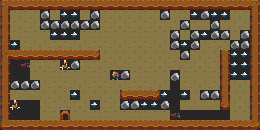
\includegraphics[scale=0.6, valign=c]{WarpedImages/boulderdashDefault.png}} \quad
  \subfloat[Warped Screen Observation for Boulderdash]{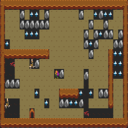
\includegraphics[scale=0.6, valign=c]{WarpedImages/boulderdashWarped.png}} \qquad
  \subfloat[Raw Screen Observation for Ikaruga]{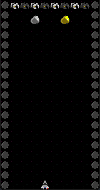
\includegraphics[scale=0.6, valign=c]{WarpedImages/ikarugaDefault.png}} \quad
  \subfloat[Warped Screen Observation for Ikaruga]{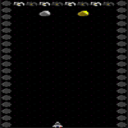
\includegraphics[scale=0.6, valign=c]{WarpedImages/ikarugaWarped.png}\label{fig:ikarugaWarped}}
  \caption{Comparison of Raw Screen Observations and Warped Screen Observations for two games}
  \label{fig:ScreenWarping}
\end{figure*}
Figure~\ref{fig:ScreenWarping} shows the effects of screen warping to a fixed size of 128x128 across a couple of games.
While it can be seen that some raw pixel information is lost during the process, elements of the games can still be seen and recognised as the down sampling effect isn't too dramatic.
Specifically as each game is made up of sprites and tiles and the warping doesn't reduce past a tile size, each tile can still be recognised.
Some games will have parts of the image up sampled as can be seen in figure~\ref{fig:ikarugaWarped}, where the x dimension has been up sampled.
\par
An advantage of applying some down sampling during the image warping process is the reduction of GPU VRAM needed during training.
As the images are physically smaller in size they take up less VRAM when stored on the GPU during each backpropagation step.
This value can then be tuned to allow for larger minibatches without overfilling the GPU VRAM.
This provides the benefit of allowing more parallel environments to run simultaneous, potentially speeding up training, and better GPU utilisation during training.

\subsection{Requiring Fixed Sized Input to the Model}
\label{ssec:fixedOutput}
As with the limitations for inputs to a neural network size, pointed out in section~\ref{ssec:fixedInput}, the output of a MLP needs to be a predetermined fixed size.
This is an issue as the number of accepted control inputs for games in the GVGAI framework vary from game to game.
\subsubsection{Action Representation in the GVGAI Framework}
Currently all of the games in the GVGAI framework use a combination of the following 6 actions:
\begin{multicols}{2}
\begin{itemize}
    \item Do Nothing
    \begin{itemize}
        \item ACTION\_NIL
    \end{itemize}
    \item Perform Action
    \begin{itemize}
        \item ACTION\_USE
    \end{itemize}
    \item Movement Actions
    \begin{itemize}
        \item ACTION\_LEFT
        \item ACTION\_RIGHT
        \item ACTION\_DOWN
        \item ACTION\_UP
    \end{itemize}
\end{itemize}
\end{multicols}
Games such as aliens (a space invaders style game) don't accept the actions ACTION\_UP and ACTION\_DOWN due to the lack of vertical movement in the game, therefore it only accepts 4 possible actions.
\par
Specifically in the GVGAI framework, these actions are represented as an integer number between 0-N exclusive where N is the total number of valid actions for that particular game.
Alongside the state observation at each time step, agents are given a list of available actions where the agent needs to return the list index of the action it wants to perform.
If an agent returns an invalid action ID then the agent is disqualified from that run, so there is a high penalty for trying to perform an invalid action.

\subsubsection{Creating a Fixed Output Layer Size}
As with the input layer of the neural network, the output layer has to be a fixed predetermined size.
To ensure the model can return actions for all games, the output of the model could be fixed to return an integer value between 0-6 exclusive.
\par
This would allow for an agent using this model to play approximately 40\% of the available games in the GVGAI framework, those that use all 6 actions.
This gives complications in the remaining 60\% of games that have a lower number of acceptable actions, as giving an invalid action at any time results in disqualification.
\subsubsection{Dropping Invalid Actions}
The proposed solution for dealing with games with a lower number of valid actions is for the agent to simply ignore invalid actions and send a ACTION\_NIL instead.
This can be achieved by comparing the action ID proposed with the length of the list of actions, dropping the action if its value is greater than or equal to the length of the list.
If an action is chosen to be dropped the agent can send the value of 0 as this corresponds to ACTION\_NIL for all games in the GVGAI framework.
\par
Doing nothing makes sense as the default state of the agent as it typically has the least impact on the state of the game.
Performing ACTION\_NIL is currently used as a way to penalise agents in the GVGAI game playing tracks that don't return an action within a given time frame without drastically going over time to result in disqualification.
This behaviour is also indicative of human play as humans don't have the reactions required to press a unique button every frame, so in human play most of the time no action is performed.
\subsubsection{Robustness of Dropping Invalid Actions}
While this method works for all current games in the GVGAI framework, it isn't robust to 2 changes to in future games due to a couple of assumptions made.
\par
The first assumption is that the maximum number of actions across all games is 6.
If a game was introduced with $>6$ actions the agent would never be able to use the actions corresponding to values~$>6$.
Although not using these actions wouldn't be grounds for disqualifying the agent, it would severely limit the agents ability to play those games as it doesn't have access to all the possible actions.
\par
The second assumption is that the action corresponding to the ID 0 is ACTION\_NIL.
Breaking this assumption could lead to unknown effects in many games depending on what the action that ID 0 mapped to.
During the learning phase it is theoretically possible that the agent could learn to not use these actions if they are detrimental to its progress.
\par
A final issue with this method is that the same ID values don't map to the same actions.
For example in Aliens action id 1 corresponds to ACTION\_USE, but in Camel Race this corresponds to ACTION\_LEFT.
This could be fixed by using the list of actions provided to the agent to translate between the model and the output, although this wasn't examined.

\subsection*{Combining Image Warping and Dropping Actions}
Through combining the methods in section~\ref{ssec:fixedInput} and section~\ref{ssec:fixedOutput} an agent with a single model can technically play all games and levels in the GVGAI framework.
This also allows for the neural network architecture to be designed separately to the agent and irespective of the games it can play.
The agent simply needs to know the input size the neural network requires to reshape the raw observation before feeding it through the neural network.

\subsection{Removing the Alpha Channel}
The raw state observation image that the agent receives is encoded as an 8-bit RGBA image.
Inclusion of an alpha channel in the raw state observation image doesn't make logical sense as typically a game doesn't have any transparency elements.
\par
After doing some analysis of all levels in the GVGAI framework it was determined that the alpha channel was redundant information.
For most of the games in the GVGAI framework the alpha channel isn't used, with the it simply being filled with 0s.
For the few games that do use the alpha channel the only values used are max (255) and zeros.
\par
The alpha channel is mostly used to show the locations of floors and walls in a maze-like games, something which is encoded in the RGB channels of the image too.
When a human player plays a game this information wouldn't be shown to them so inclusion of the alpha channel could also be seen as giving extra knowledge to the agent.
\par
The alpha channel was therefore removed from the raw state observation images by simply slicing it off before feeding it through the model.
This is done to reduce the dimensionality of the input data, allowing for few parameters needed to be learnt and quicker processing of the state observations.

\subsection{Scaling Rewards During Training}
While all the previous processing techniques are performed during both training and playing, this technique is only used during training to help normalise the rewards across all of the games.
Normalisation is a common technique used in machine learning to help speed up the training process.
The requirement for such a technique is motivated from how some games have higher or more frequent rewards than others.
\par
Mnih et al.~\cite{DeepAtari} tackled this by clipping all positive rewards to 1 and negative rewards to -1 when training on Atari games.
The authors mentioned that this `limits the scale of the error derivatives and makes it easier to use the same learning rate across multiple games', a useful feature for general video game playing.
They continued to suggest how this method could effect performance of the agent as `it cannot differentiate between rewards of different magnitude.'
\par
The method proposed here aims to tackle both the issue of higher total rewards, and more frequent rewards while retaining the ability to differentiate between different reward magnitudes.
To do this, all the rewards are scaled by a fraction of the maximum score achievable in that game.
\par
The scaled rewards are calculated by the following equation
\begin{equation} \label{eq:scalingReward}
    r\prime=r\times\frac{k}{m}
\end{equation}
Where $r\prime$ is the scaled reward, $r$ is the given reward, $k$ is the scaling factor, and $m$ is the maximum possible score in that level.
This also has the added benefit of showing how far off obtaining a perfect score an agent is during training by plotting the episode rewards, a common metric tracked in reinforcement learning.
\par
The use of the maximum score during training can be seen as a domain specific knowledge as it requires analysis of the game and levels used during training to figure out the maximum achievable score.
While this is true, at no point is the underlying model exploiting this domain specific knowledge with it being used to give equal priority to all games in the training set.

\subsection{Agent Structure}
These methods and the neural network model are integrated together in the form of an intelligent agent.
The overall agent can be classified as a purely reactive agent, without any internal memory.
At each time step the agent perceives the game via the raw screen image, which is processed to remove the alpha channel and warp to a fixed size before being processed by the underlying CNN which drives the agents decision making.
The action chosen by the CNN is checked to see if its a valid action and dropped if necessary, passing the final action decision onto the environment.
Figure~\ref{fig:agentStructure} shows this relationship diagrammatically.
\begin{figure}[h]
  \centering
  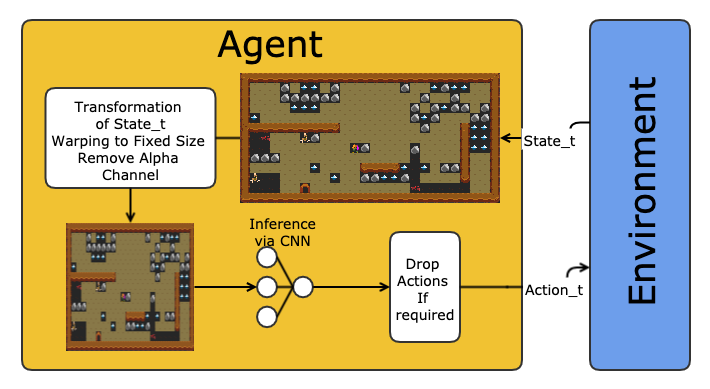
\includegraphics[width=0.7\linewidth]{figures/agentStructure.png}
  \caption{Agent Structure Diagram}
  \label{fig:agentStructure}
\end{figure}

\section{Experiments}
\begin{figure*}[ht]
  \centering
  \subfloat[][Average Scores w/ StDev Error Bars]{
    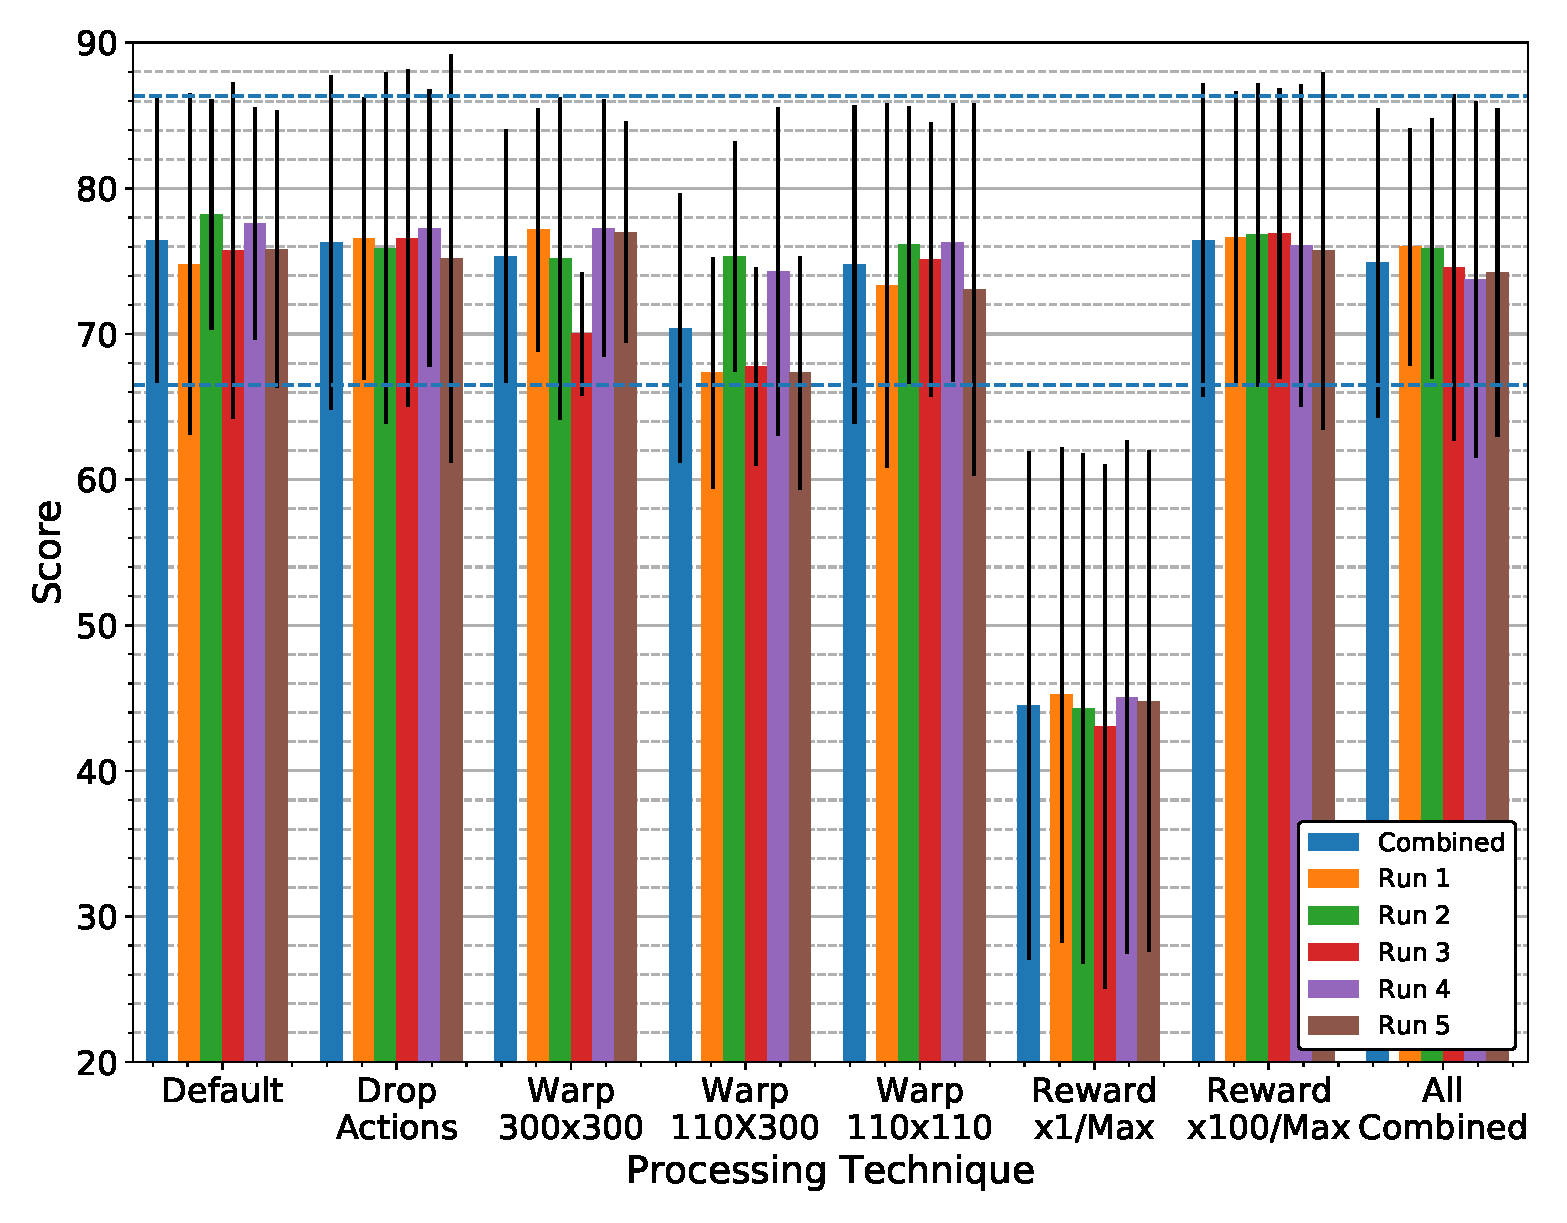
\includegraphics[width=0.45\linewidth]{graphs/Scores.eps} \label{fig:ProcessingA}
  }
  \subfloat[][Win\% w/ $\pm5\%$]{
    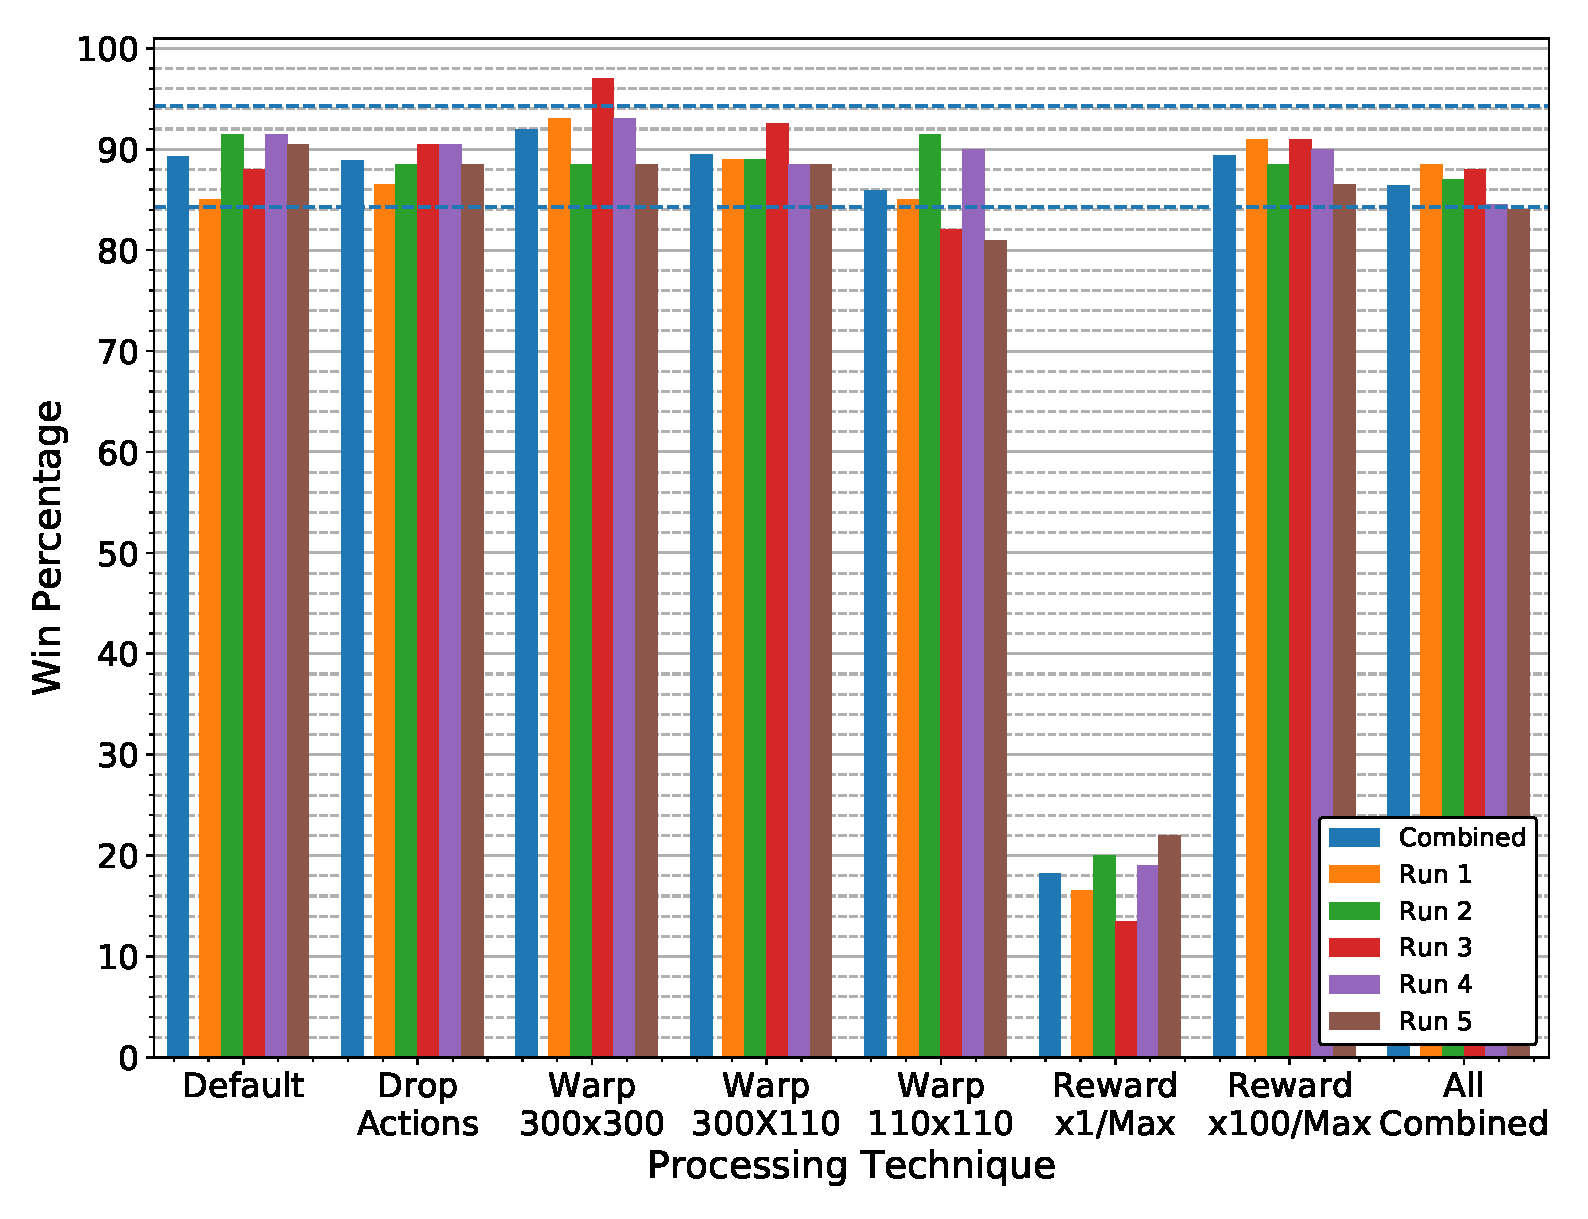
\includegraphics[width=0.45\linewidth]{graphs/Wins.eps} \label{fig:ProcessingB}
  }
  \caption{Performance Comparisons of the Different Methods Tested}
  \label{fig:Processing}
\end{figure*}
The main 3 methods presented were tested to show they aren't negatively effecting performance of the agent when trained with these adaptations. 
Due to the simplicity of the technique, removal of the alpha channel was applied to all of the experiments.
Each of the methods were tested against a agent trained with default settings, and where possible a few hyperparameters for each method were tried.
A final run was also tested which included a combination of all of the methods together.

\subsection{Experimental Method}
\label{ssec:experimentalMethod}
All of the agents were trained and tested on level 1 of the game aliens, to show that the methods don't effect performance of a agent designed to play a single known level - a known successful application of reinforcement learning.
Level 1 of aliens was chosen as it has properties required to test all of the methods and performance can be loosely compared to the results from the initial investigations by Torrado et al. when applying deep reinforcement learning to the GVGAI framework~\cite{GVGAIGym}. 
While any game could serve a decent test for raw state observation image warping, Aliens also has 4 actions due to no vertical movement and a large maximum score with positive rewards of differing magnitudes.
\par
As a efficient and popular modern reinforcement learning algorithm, Advantage Actor-Critic (A2C) was used to test all of the methods.
The implementation for this algorithm came from the Stable Baseline library, a simpler fork of the OpenAI Baseline library~\cite{stable-baselines}.
The model architecture and other hyperparameters were the same as used by Torrado et al. during their introduction of the GVGAI Gym framework~\cite{GVGAIGym}, apart from training time which was increase to ten million frames of gameplay to allow to results on long term performance and convergence to be seen.
As the convergence process of stochastic gradient descent learning is inherently random, five models with each adaptation were trained.

\subsection{Method Hyperparameters Tested}
This section aims to give a brief explanation of the hyperparameters of each adaptation that was tested.
\subsubsection{Dropping Actions}
Dropping unacceptable actions was tested with a model output of size 6 where as aliens only accepts 4 actions.
\subsubsection{Image Warpping}
Three different screen warps were tested. The original screen size is 300x110 so this was used as the basis for screen decisions.
300x300 allows for no loss of data but creates a much larger model, 110x300 creates the same size of model as default but still warps the image, 110x110 will only warp the image in the y direction squishing it from 300 to 110.
\subsubsection{Scaling Rewards}
Two different reward scaling factors were tested, one by a factor of $\frac{1}{Max}$ and another by $\frac{100}{Max}$.
The maximum possible score for Aliens level 1 was determined to be 87 through analysis of the game rules and level layout.
\subsubsection{All Combined}
\label{sssec:allCombined}
Finally a combination of all the processing techniques were used in a final experiment, with 110x110 used for image warping and $\frac{100}{Max}$ for the reward scaling factor.

\subsection{Results and Evaluation}
\subsubsection{Performance Graphs}
The graphs in Figure~\ref{fig:Processing} shows the average score and win\% of each of the trained models over 100 games played, in the 5 grouped bars for each method.
The preceding bar shows the combined performance when joining the results from all 5 models trained with that adaptation together.
\par
Figure~\ref{fig:ProcessingA} shows that that the majority of the methods used score within 1 standard deviation of the combined default average score.
Similar results can be seen when comparing the win\% in Figure~\ref{fig:ProcessingB}, again the majority of the methods lie with in a narrow margin of the combined default win\% with $\pm$ 5\% being marked on the graph.

\subsubsection{Low Performance of Reward Scaling by $\frac{1}{Max}$}
The only method that performed badly was scaling the rewards by $\frac{1}{Max}$, with it clearly being an outlier to all the other methods and the default configuration.
The resulting agent performs similarly to a purely random agent, and looking at training metrics it suggests that the model struggled to learn throughout the training process.
This could be attributed to vanishing gradients during training, this occurs when the weight updates for each minibatch are insignificant and the model doesn't learn due to the small gradients received, which could be due to the small rewards given.
Changing hyperparameters such as learning rate could mitigate this but as a reward scaling of $\frac{100}{Max}$ has proven to be effective this wasn't investigated.
\subsubsection{Conclusion}
These results show that these methods do not negatively impact performance on single game playing.
By using the combination of input and output processing, any game can be processed by the model to allow GVGP, while employing reward scaling cross game training can happen more effectively.


\section{Evaluation of GVGP Performance}
To evaluate the combination of these methods in the context of GVGP, the competition parameters of the 2018 GVGAI Learning track were used.
More information about these rules can be found in the 2019 GVGAI survey\cite{GVGAI19}.
As the validation levels for the 2018 track haven't been released at the time of writing, 3 games from the set were chosen to run be the games to train and test on.
\par
The chosen games were Aliens, Missile Command and Boulderdash.
These games were chosen based upon the results of the initial paper for the GVGAI gym framework by Torrado et al.\cite{GVGAIGym}.
While Torrado et al. used the same network and hyperparameters during training, they trained each game separately and only trained upon a single level.
This gives a good starting point to show what games and hyperparameters could work well for general video game playing.
\par
For each of the games levels 0 and 1 were used for training and levels 2,3 and 4 were used for validation.
The same settings were used as in section~\ref{ssec:experimentalMethod} while trained for 100 million frames of gameplay with the same combined parameters described in section~\ref{sssec:allCombined}, these resulting network is labelled model 1.
A further 2 models were trained based off the VGG16 architecture first described by Simonyan and Zisserman as an example of how current deep CNNs work~\cite{VGG16}.
The both used a screen warping size of 128x128 and both trained for less time before plateauing, at 17 million and 10 million time-steps, for model 2 and 3 respectively.
Model 3 uses the same architecture described by Simonyan and Zisserman~\cite{VGG16} only changing the output layer to the desired size.
Model 2 used the same feature extraction as VGG16 but has fewer nodes in the hidden MLP layers at 128 and 64. 

\subsection{Qualitative Results}
In this section the performance of the final trained agent is evaluated qualitatively by running the trained agent in both the training and validation levels.
\subsubsection{Aliens}
Performance on Aliens was quite interesting, while the agent performed well it struggled to shoot the aliens with the precision that you might expect from perfect play.
This could be due to how the agent has no perception of time and therefore the speed and direction the aliens are moving at.
\par
Its ability to shoot down aliens degrades the further the aliens appear down the screen, which could be due to it having little experience in those situations.
While all levels currently available have the aliens spawn in the upper left hand corner of the screen, aliens spawning elsewhere could be a problem to this agent.
\par
As the barriers provide points for destroying them the agent employs a rather reckless strategy of getting rid of its defensive to maximise points while simply dodging all incoming missiles.
\subsubsection{Missile Command}
\label{sssec:qualMC}
During the training levels of missile command there are only red missiles that the agent has to stop where as in the validation levels 2 and 3 there are blue missiles too.
In these levels the agents just ignore the blue missiles as it has never seen these before, resulting in some negative points and loses.
Level 4 is relatively similar to level 1 which explains why the agents perform well on it again.
\subsubsection{Boulderdash}
All agents struggled to win boulderdash due to win condition not having a reward associated with it.
It appeared that the agents significantly over fit to the 2 training levels with the agents appearing to move in a set pattern.
This meant that in one of the validation levels the agent tried to continuously move upwards even though it was at the top of the screen, this repeated behaviour also signifies a disadvantage of a purely reactive agent and architecture as, due to the state of the game not visually changing, the agent kept repeating the same useless action.
As a result the agents couldn't scored very poorly on the validation levels for boulderdash, showing it failed to generalise to new levels.
\subsubsection{All Games}
Unlike the planning agents there is no expectation that these agents could generalise to other games in the GVGAI framework as they haven't learnt to play them.
This puts these agents at a significant disadvantage currently compared to the vastly more general planning agents.
This effect can be seen as the competition organisers only expect the learning agents to perform in 3 games vs the 10 games that planning agents are evaluated in.

\subsection{Comparison with planning agents}
These three games were featured together in the GVGAI training set 1 for planning agents\cite{GVGAITrainingSet1} and was used during the CIG 2014 and 2015 GVGAI competitions.
As such planning agents created for these competitions (as well as other agents evaluated on the training set) can be downloaded and used to compare against.
Unfortunately at the time of writing there are no agents from the learning track that are available to download and run.
As the winner of the 2014 competition adrienctx was chosen as the agent to compare to, alongside a sample MCTS method and a random agent.

\subsection{Quantitative Results}
The graph in Figure~\ref{fig:aliensScore} compares the average score for all agents over 10 playthroughs of each level.
Note the dotted vertical line separates the training and test levels for the models.
\begin{figure}[ht]
  \centering
  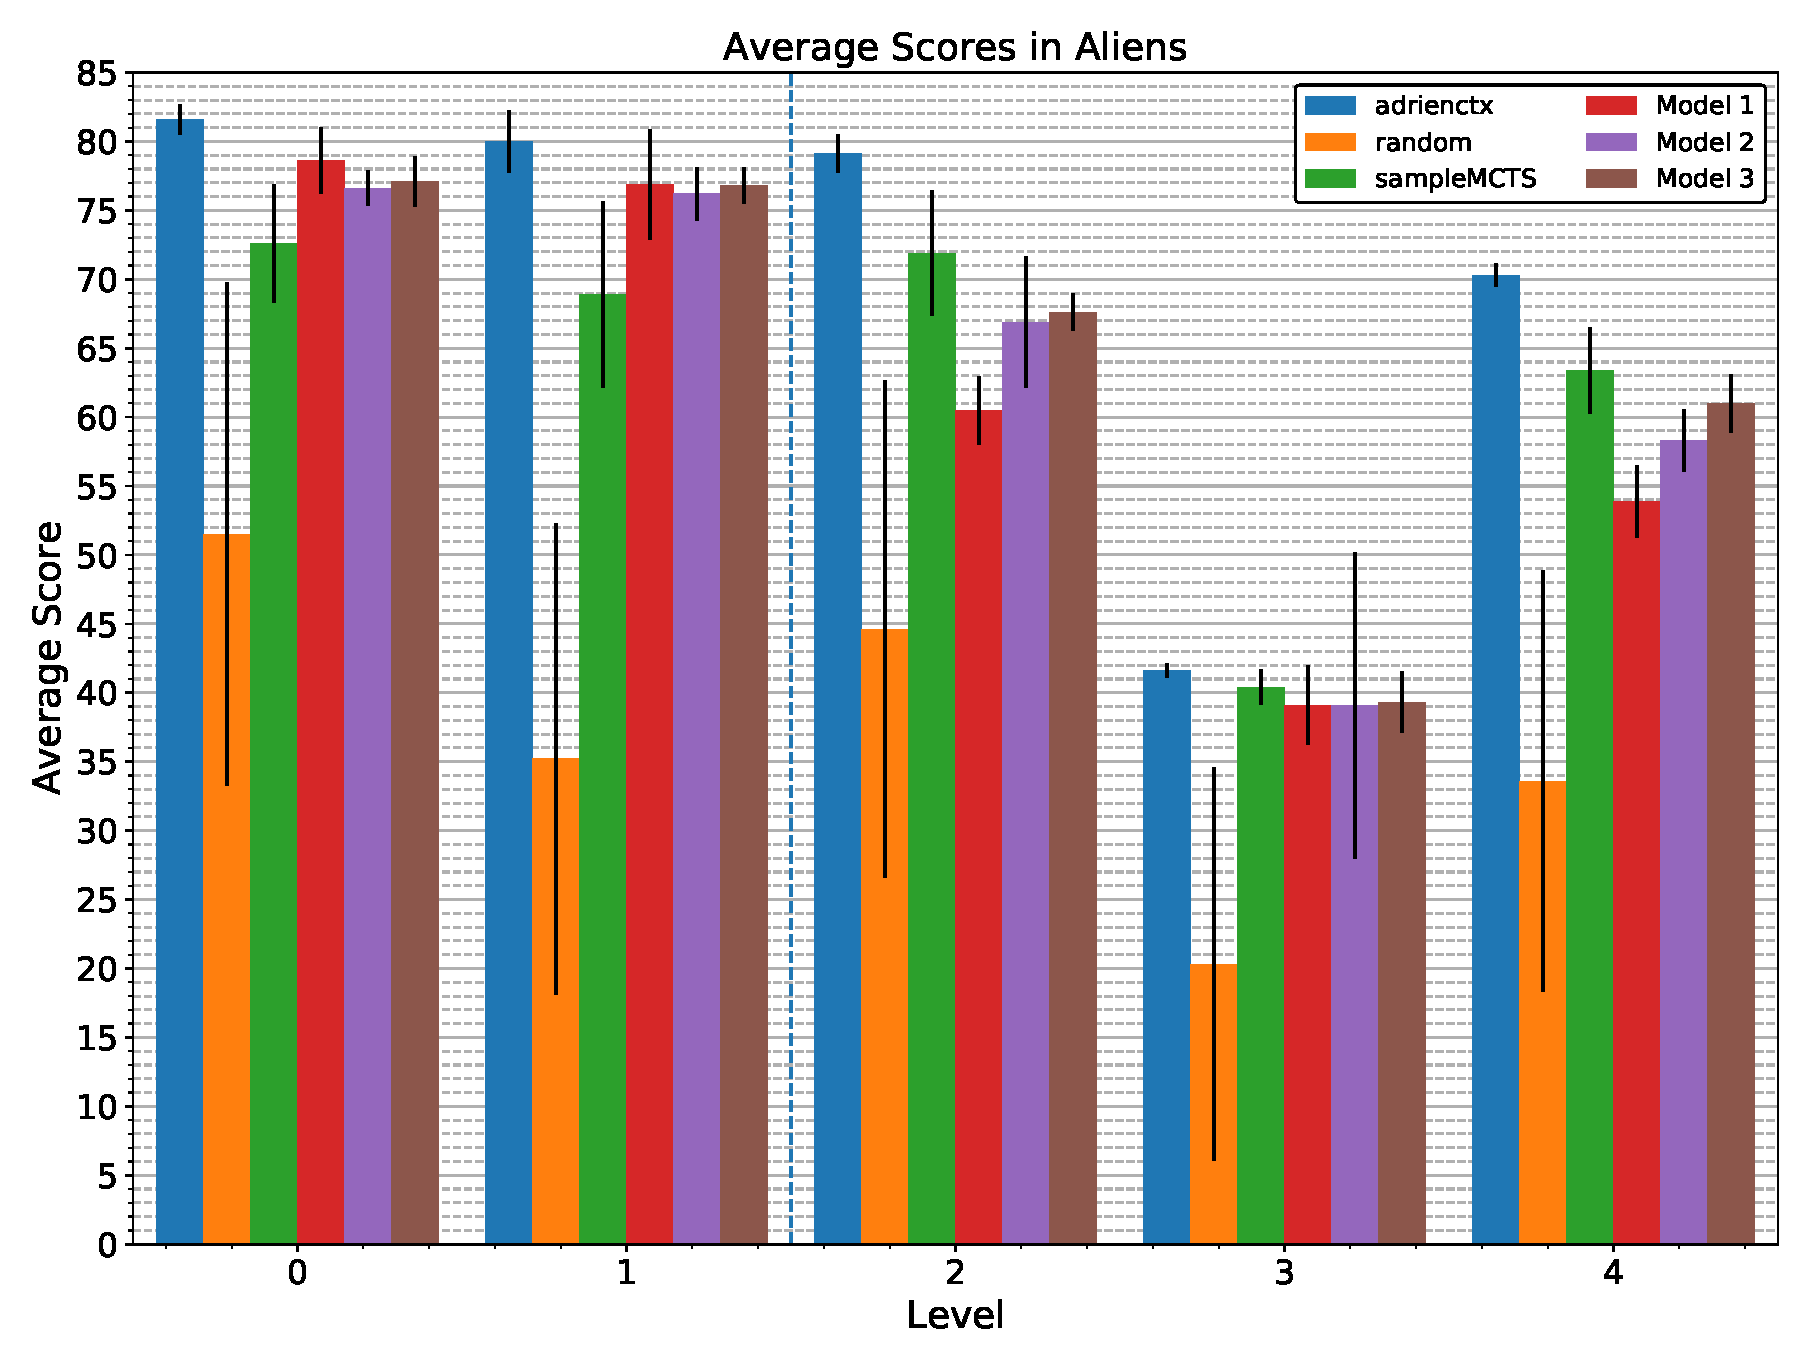
\includegraphics[width=0.7\linewidth]{graphs/FinalAliensScores.eps}
  \caption{Performance Comparisons with previous Agents}
  \label{fig:aliensScore}
\end{figure}
\par
While aliens was the closet game it is still clear that the planning agents have a slight advantage.
In Boulderdash acrienctx was the clear winner as it was the only agent to achieve wins on all 5 levels, but in Missile Command the model agents performed best, on levels 0,1 and 4 but couldn't win levels 2 and 3 due to the ignoring of blue missiles discusses in Section~\ref{sssec:qualMC}.
\par
An interesting point is that while running the model on a GTX 1080 GPU, the inference time of the model was approximately 5-8ms, significantly lower than the 40ms planning agents needed.
This would allow agents to play games at above 60fps vs the 24fps current planning agents play at, which is more comparable to the arcade games the GVGAI framework is based upon.


\section{Conclusion}
Neural networks have shown promise in both general AI problems and the application of video game playing, with nothing to suggest they can't achieve similar high levels of performance on general video game playing.
Due to the limitations of neural networks GVGP applications were hard to test due to the fixed input and output sizes required.
Solving these issues allows us to benefit from diverse range of neural network architectures and the benefits of them compared to planning based agents.

\subsection{Neural Network Based Agents}
The main benefit is agents don't rely on a forward model, something which Levine et al. suggested would be interesting when they proposed a GVGP competition~\cite{GVGP}.
In complex modern games, a forward model might not be accessible or could be too computationally demanding to use effectively in search based agents due to less time to generate tree nodes.
Games with imperfect information, or many random/non-deterministic elements (such as opponent players) can also cause problems with using a forward model based approach.
\par
Although approaches for modern video game playing exploit access to raw games state~\cite{OpenAIFive, alphastarblog}, it has been shown that CNNs agents can learn to play games from screen observations.
This brings agents inline with the information that human players have access too, and allows games to be played where you don't have access to the game state such as unmodified commercial titles.
\par
A final major benefit of model based agents is that they have a fixed inference time.
This allows for designers to be confident that an action will be chosen on time, allowing for strict deadlines such as frame times to be adhered too with high confidence.
If the the computation time changed due to weaker hardware or playing games with a higher framerate, a neural network could perform equally as well so long as it had enough inference time where as a planning based agent would suffer as it couldn't search as deep.
\par
As with all neural network based agents, the lack of explainability can be considered a downside.
At their best neural networks can only be interpreted and its hard to predict how they would perform on new games or changes to current games.
Another downside is the large file size of models and memory requirements compared to planning agents, limiting their usefulness in situations like opponent AI in a smart phone app.

\subsection{Future Work}
This paper shows novel methods to allow for cross game training for GVGP learning agents that use a neural network, this allows us to benefit from the quickly growing field of reinforcement learning for GVGP.
It is clear that training methods still need to be improved if agents are going to perform as well as their planning based counter parts.
There is room for exploring more complex network architectures such as recurrent neural networks or giving the agent a series of previous frames to show change in the state.
Methods for expanding the agents playable games through transfer learning could allow for more general game playing.
Procedural content generation could help alleviate the overfitting of the training levels by providing a wide distribution of levels to train in, something that is been initially investigate by Justesen et al.~\cite{PCG}.

% if have a single appendix:
%\appendix[Proof of the Zonklar Equations]
% or
%\appendix  % for no appendix heading
% do not use \section anymore after \appendix, only \section*
% is possibly needed

% use appendices with more than one appendix
% then use \section to start each appendix
% you must declare a \section before using any
% \subsection or using \label (\appendices by itself
% starts a section numbered zero.)
%


% \appendices
% \section{Proof of the First Zonklar Equation}
% Appendix one text goes here.
%
% % you can choose not to have a title for an appendix
% % if you want by leaving the argument blank
% \section{}
% Appendix two text goes here.

% \section*{Acknowledgments}
%  The authors would like to thank our colleagues from The University of Nottingham for their insights into the project during its development.

%, with particular thanks to Timothy Cargan for their tremendous insights into the field.

% Can use something like this to put references on a page
% by themselves when using endfloat and the captionsoff option.
\ifCLASSOPTIONcaptionsoff
  \newpage
\fi



% trigger a \newpage just before the given reference
% number - used to balance the columns on the last page
% adjust value as needed - may need to be readjusted if
% the document is modified later
%\IEEEtriggeratref{8}
% The "triggered" command can be changed if desired:
%\IEEEtriggercmd{\enlargethispage{-5in}}









% references section
\bibliographystyle{IEEEtran}
\bibliography{main}







% biography section
%
% If you have an EPS/PDF photo (graphicx package needed) extra braces are
% needed around the contents of the optional argument to biography to prevent
% the LaTeX parser from getting confused when it sees the complicated
% \includegraphics command within an optional argument. (You could create
% your own custom macro containing the \includegraphics command to make things
% simpler here.)
%\begin{IEEEbiography}[{\includegraphics[width=1in,height=1.25in,clip,keepaspectratio]{mshell}}]{Michael Shell}
% or if you just want to reserve a space for a photo:

% \begin{IEEEbiography}{Michael Shell}
% Biography text here.
% \end{IEEEbiography}

% % if you will not have a photo at all:
% \begin{IEEEbiographynophoto}{John Doe}
% Biography text here.
% \end{IEEEbiographynophoto}

% % insert where needed to balance the two columns on the last page with
% % biographies
% %\newpage

% \begin{IEEEbiographynophoto}{Jane Doe}
% Biography text here.
% \end{IEEEbiographynophoto}

% You can push biographies down or up by placing
% a \vfill before or after them. The appropriate
% use of \vfill depends on what kind of text is
% on the last page and whether or not the columns
% are being equalized.

%\vfill

% Can be used to pull up biographies so that the bottom of the last one
% is flush with the other column.
%\enlargethispage{-5in}



% that's all folks
\end{document}
